\begingroup
\newcommand{\GerlingSeptSeconds}[2]{#1\makebox[.42em][c]{,\makebox[0pt][r]{\textsuperscript{s}}}#2}
\begin{center}
\textsc{Gauss} an \textsc{Gerling}.\quad Göttingen, 1.~September 1823.
\end{center}

\par\noindent\hspace*{\parindent}\mbox{.\ .\ .\ .\ .\ .\quad Ich} habe Ihnen nur mein Verfahren beim Telegrafieren beschrieben. Die Zahlenzeichen haben ebenso wenig bestimmte, feste Werte wie \(a\) und \(x,y,z\) in der Algebra. Ihre Bedeutungen werden immer für die Umstände, die sich im Voraus erwarten lassen, vorab vereinbart.
Ich befürchte allerdings, dass das Telegrafieren zumindest mit dem Meisner-Heliotrop sehr unzuverlässig wäre, denn er scheint mir sehr schlecht justiert zu sein.
Besonders in der Stunde von 2---3\textsuperscript{h} (in der die anderen Gegenstände gewöhnlich zu stark flimmern, um etwas Brauchbares messen zu können)\textsuperscript{*}) habe ich stets festgestellt, dass das Licht plötzlich abbricht, wenn es am hellsten leuchtet, dann eine Zeit lang ganz unsichtbar bleibt, darauf nach und nach als winziger Lichtpunkt wieder erscheint und erst zuletzt seine volle Helligkeit erreicht, sie aber leider nur kurze Zeit \textls[120]{behält} (manchmal nur \(\frac{1}{4}\) Minute). Unter solchen Umständen ist an zuverlässiges Telegrafieren nicht zu denken.
\par\smallskip\noindent\rule{.24\linewidth}{.4pt}\par\nobreak
{\footnotesize\noindent\hspace*{\parindent}\textsuperscript{*}) Zwischen 6 und 7\textsuperscript{h} habe ich das Licht nämlich seltener beobachtet, weil ich keine Zeit zum Messen verlieren wollte.\par}
\smallskip\noindent\hfill{\small49\textsuperscript{*}}\hspace*{.123\linewidth}\par
\clearpage
\noindent\makebox[0pt][l]{\fontsize{13}{16}\selectfont 388}\hfill{\small\textbf{BRIEFWECHSEL MIT GERLING.}}\hfill\null\par\medskip
\par\noindent\hspace*{\parindent}Ich hatte 1822 einen ähnlichen Fall mit dem ältesten Heliotrop, der sich damals auf dem Deister befand und dessen Justierung vermutlich durch unsanften Transport gelitten hatte.
Ich half mir damals mit einer Behelfslösung.
Wir stellten nämlich wiederholt Versuche an, indem ich zuerst dem Leutnant \textsc{Hartmann} durch ein bestimmtes Zeichen zu verstehen gab, \textls[120]{dass} die Versuche gemacht werden sollten.
Dann ließ er das Sonnenbild wiederholt in verschiedenen Höhen durch das Fadenkreuz gehen,
\par\vspace{.7cm}
{\centering
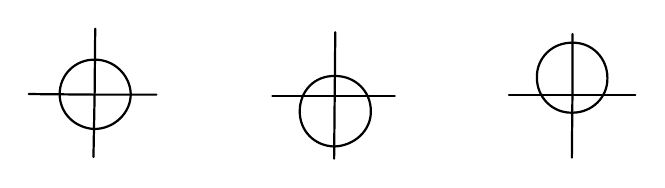
\begin{tikzpicture}[x=.0074cm,y=-.0074cm,line width=.8pt,line cap=round,line join=round]
\draw (103,151) .. controls (103,118) and (130,91) .. (164,92) .. controls (197,92) and (224,119) .. (225,151) .. controls (225,184) and (196,211) .. (162,211) .. controls (129,209) and (103,184) .. (103,151) -- cycle;
\draw (50,151)--(163,152)--(269,152);
\draw (164,39)--(163,151)--(161,259);
\draw (515,181) .. controls (515,146) and (540,119) .. (576,120) .. controls (610,120) and (637,146) .. (637,180) .. controls (638,213) and (609,240) .. (574,241) .. controls (540,240) and (515,214) .. (515,181) -- cycle;
\draw (468,154)--(575,154)--(678,154);
\draw (576,45)--(575,154)--(574,262);
\draw (922,123) .. controls (921,89) and (949,62) .. (983,63) .. controls (1017,62) and (1043,90) .. (1043,123) .. controls (1044,157) and (1016,183) .. (983,183) .. controls (949,184) and (922,157) .. (922,123) -- cycle;
\draw (874,153)--(983,153)--(1091,153);
\draw (983,48)--(983,153)--(982,260);
\end{tikzpicture}\par}
\vspace{.7cm}\noindent und ich zeigte ihm den Augenblick, in dem ich sein Licht zum ersten Mal in voller Helligkeit sah, durch Öffnen meines Heliotrops an und das Ende der vollen Helligkeit durch Abdecken.
Es versteht sich, dass die Sonne dabei immer fast genau in der Mitte des Fadenkreuzes meines Heliotrops stand, damit ich ganz sicher sein konnte, dass mein Licht dort in voller Stärke ankam.
Auf meiner Seite waren also 3 Personen nötig: eine, die den Heliotrop immer fast genau zentriert hielt, eine zweite, die mit dem Fernrohr (die Entfernung betrug \(8\frac{1}{2}\) Meilen) den Heliotrop auf der anderen Seite beobachtete, und eine dritte, die auf den Zuruf der zweiten den Spiegel des Heliotrops freigab oder abdeckte (einfach indem sie vor ihn trat).
Das würde ich auch mit Ihnen sehr gern tun.
Das 3-fache Aufmerksamkeitszeichen (\GerlingSeptSeconds{1}{2} geschlossen, \GerlingSeptSeconds{1}{2} offen, \GerlingSeptSeconds{1}{2} geschlossen usw.\ usw.) könnte anzeigen, dass man den Versuch vorhat (den man nur macht, wenn kaum eine Abdeckung durch Wolken zu befürchten ist). Dabei gibt derjenige das Zeichen zuerst, der den Heliotrop des anderen prüfen will.
Da sich Gelehrten leicht predigen lässt, brauche ich wohl nichts darüber hinzuzufügen, wie man die Versuche nutzt.
Bei ähnlicher Winkelstellung ist dieses Mittel fast so gut wie eine wirkliche Justierung, da derjenige, der den geprüften Heliotrop hat, weiß, wie er das Sonnenbild durchlaufen lassen muss und ob er das Instrument umstellen muss, \textls[120]{bevor} die Sonne ausgetreten ist oder nachdem sie schon ein Stück weit ausgetreten ist usw.
Beim \textls[120]{neuen} Heliotrop ist die Justierung hoffentlich gut.
\par\noindent\hspace*{\parindent}Was Sie mir über den \textls[120]{Unterschied} zwischen Ihrer und meiner Art der Zeichengebung schreiben, ist mir nicht ganz klar.
Ganz wesentlich
\par\clearpage
\noindent\null\hfill{\small\textbf{ZUR HANNOVERSCHEN TRIANGULATION.}}\hfill\makebox[0pt][r]{\fontsize{13}{16}\selectfont 389}\par\medskip
\noindent scheint mir zu sein, dass das Aufmerksamkeitszeichen erst \textls[120]{erwidert} werden muss, bevor man das eigentliche Zeichen gibt. Ob man aber jenes und dieses Zeichen mit einem eigenen Fernrohr oder in Ermangelung eines solchen mit dem Heliotropfernrohr beobachtet, macht wohl keinen Unterschied.
\par\noindent\hspace*{\parindent}Ich habe mein Zeichenverfahren öfter geändert. Dasjenige, das ich Ihnen beschrieben habe, scheint mir am zweckmäßigsten.
Leider habe ich versäumt, mir eine Abschrift zu machen, und kann mich schon jetzt aus dem Gedächtnis allein nicht mehr ganz genau daran erinnern.
Lassen Sie mir also bitte diese Stelle meines Briefes \mbox{abschreiben.\quad.\ .\ .\ .\ .\ .}
\par
\endgroup
